\chapter{Tâche 3 — Framework de test d'intégration et de non-régression}
\label{chap:t3}
% Entreprise : Free Mobile

% =====================================================================
%  Trame conseillée (réutilisée pour chaque tâche) :
%  1. Contexte & dette technique de départ
%  2. Objectif de la mission
%  3. Conception / choix techniques
%  4. Réalisation (extraits de code COMMENTÉS, schémas — PAS de code entier)
%  5. Difficultés rencontrées
%  6. Résultats & bénéfice business (réduction de la dette)
% =====================================================================

\section{Contexte et dette technique initiale}
% TODO : avant ton arrivée, comment la non-régression était-elle gérée ?
% (tests manuels ? absence de filet de sécurité ? régressions récurrentes ?)
% Quantifier si possible le « coût » de cette dette.
La non-régression du \emph{Valo Engine} reposait initialement sur une suite de
tests écrits en Lua. Ce langage permettait de scripter des scénarios, mais ne
s'avérait pas le mieux adapté à ce que l'on cherchait à faire. Sa nature
\textbf{impérative} laissait en effet au rédacteur d'un test toute latitude pour
y introduire de la logique : un test pouvait dès lors échouer non à cause d'une
régression du logiciel testé, mais à cause d'un défaut du test lui-même. La
frontière entre code de test et code testé devenait floue, ce qui fragilisait la
confiance accordée à ce filet de sécurité. À cela s'ajoutait un couplage de bas
niveau : le protocole de communication du moteur — un protocole TCP décrit en C
— était embarqué dans le Lua, ce qui rendait la suite délicate à maintenir.

\section{Objectif de la mission}
% TODO : concevoir un framework de tests d'intégration / non-régression /
% fonctionnels pour le programme initial.
L'objectif était de remplacer cette suite Lua par un framework dédié, reposant
sur des scénarios \textbf{déclaratifs}, volontairement plus contraignants. En
restreignant fortement la forme des tests — un scénario décrit \emph{quoi}
vérifier, jamais \emph{comment} —, on garantit que l'échec d'un test, dès lors
que le framework se trouve dans une version stable, provient bien du code du
logiciel testé et non de la mécanique de test. Le nouveau framework devait au
minimum couvrir le périmètre fonctionnel déjà assuré par le Lua : la simulation
des trames d'appel (appels voix, envoi de SMS et de MMS, consommation de data)
ainsi que la vérification des données ainsi produites.

\section{Conception et choix techniques}
% TODO : architecture du framework (runner, fixtures, jeux de données,
% rapports), langage/outils retenus et pourquoi, intégration au pipeline.

La première étape a consisté à \textbf{porter en Python} le protocole TCP par
lequel le framework dialogue avec le \emph{Valo Engine}, jusque-là décrit en C
et embarqué dans le Lua. Le module \texttt{ctypes} de Python permet de définir
des structures dont la disposition binaire est strictement équivalente à celle
de leurs homologues C ; on reconstitue ainsi un échange de trames identique à
celui du moteur sans recourir au langage natif.

Le framework prend en entrée des scénarios de test rédigés en YAML. Ces
scénarios sont analysés par un \textbf{parseur SAX}, qui présente deux
avantages : il permet de récupérer la position (ligne) de chaque instruction
— information transmise au débogueur pour offrir une exécution \emph{pas à
pas} — et il interrompt l'analyse dès la première erreur de syntaxe en
indiquant sa localisation et sa nature (arguments mal formés ou instruction
non supportée).

L'exécution repose sur une \textbf{boucle séquentielle} simple : les
instructions sont jouées les unes après les autres, sans branchement ni
retour arrière. Chaque ligne de texte est transformée en objet
\emph{instruction} suivant le patron \emph{Command} : une \emph{factory}
instancie la commande correspondante à partir d'un \emph{registry} où sont
enregistrées toutes les commandes supportées.

Autour de cette boucle, le framework fournit les services nécessaires pour
\textbf{moquer} les briques avec lesquelles le logiciel testé — le
\emph{Valo Engine} — interagit : un service simulant les équipements qui
interrogent le moteur (autorisation d'appel ou de SMS, vérification du crédit
selon la localisation) et un service recevant les notifications de seuil
émises par le moteur (courriels et messages). Enfin, un ensemble
d'instructions de \textbf{vérification} contrôle, pour une trame d'appel
donnée, la cohérence des données générées en base.

Le mécanisme de vérification reprend le principe de \emph{snapshot} déjà employé
côté Lua : les actions jouées ainsi que l'état final de la base de données sont
sérialisés, puis comparés à une trace de référence enregistrée lors d'une
exécution validée ; toute divergence signale une régression. Pour disposer
d'emblée d'une restitution des résultats exploitable — comptes rendus,
agrégation des échecs, comparable à celle d'une suite de tests classique — le
framework a été bâti comme une \textbf{surcouche de Pytest}, la génération et la
comparaison des snapshots étant déléguées à la bibliothèque \textbf{syrupy}.

\begin{figure}[H]\centering
  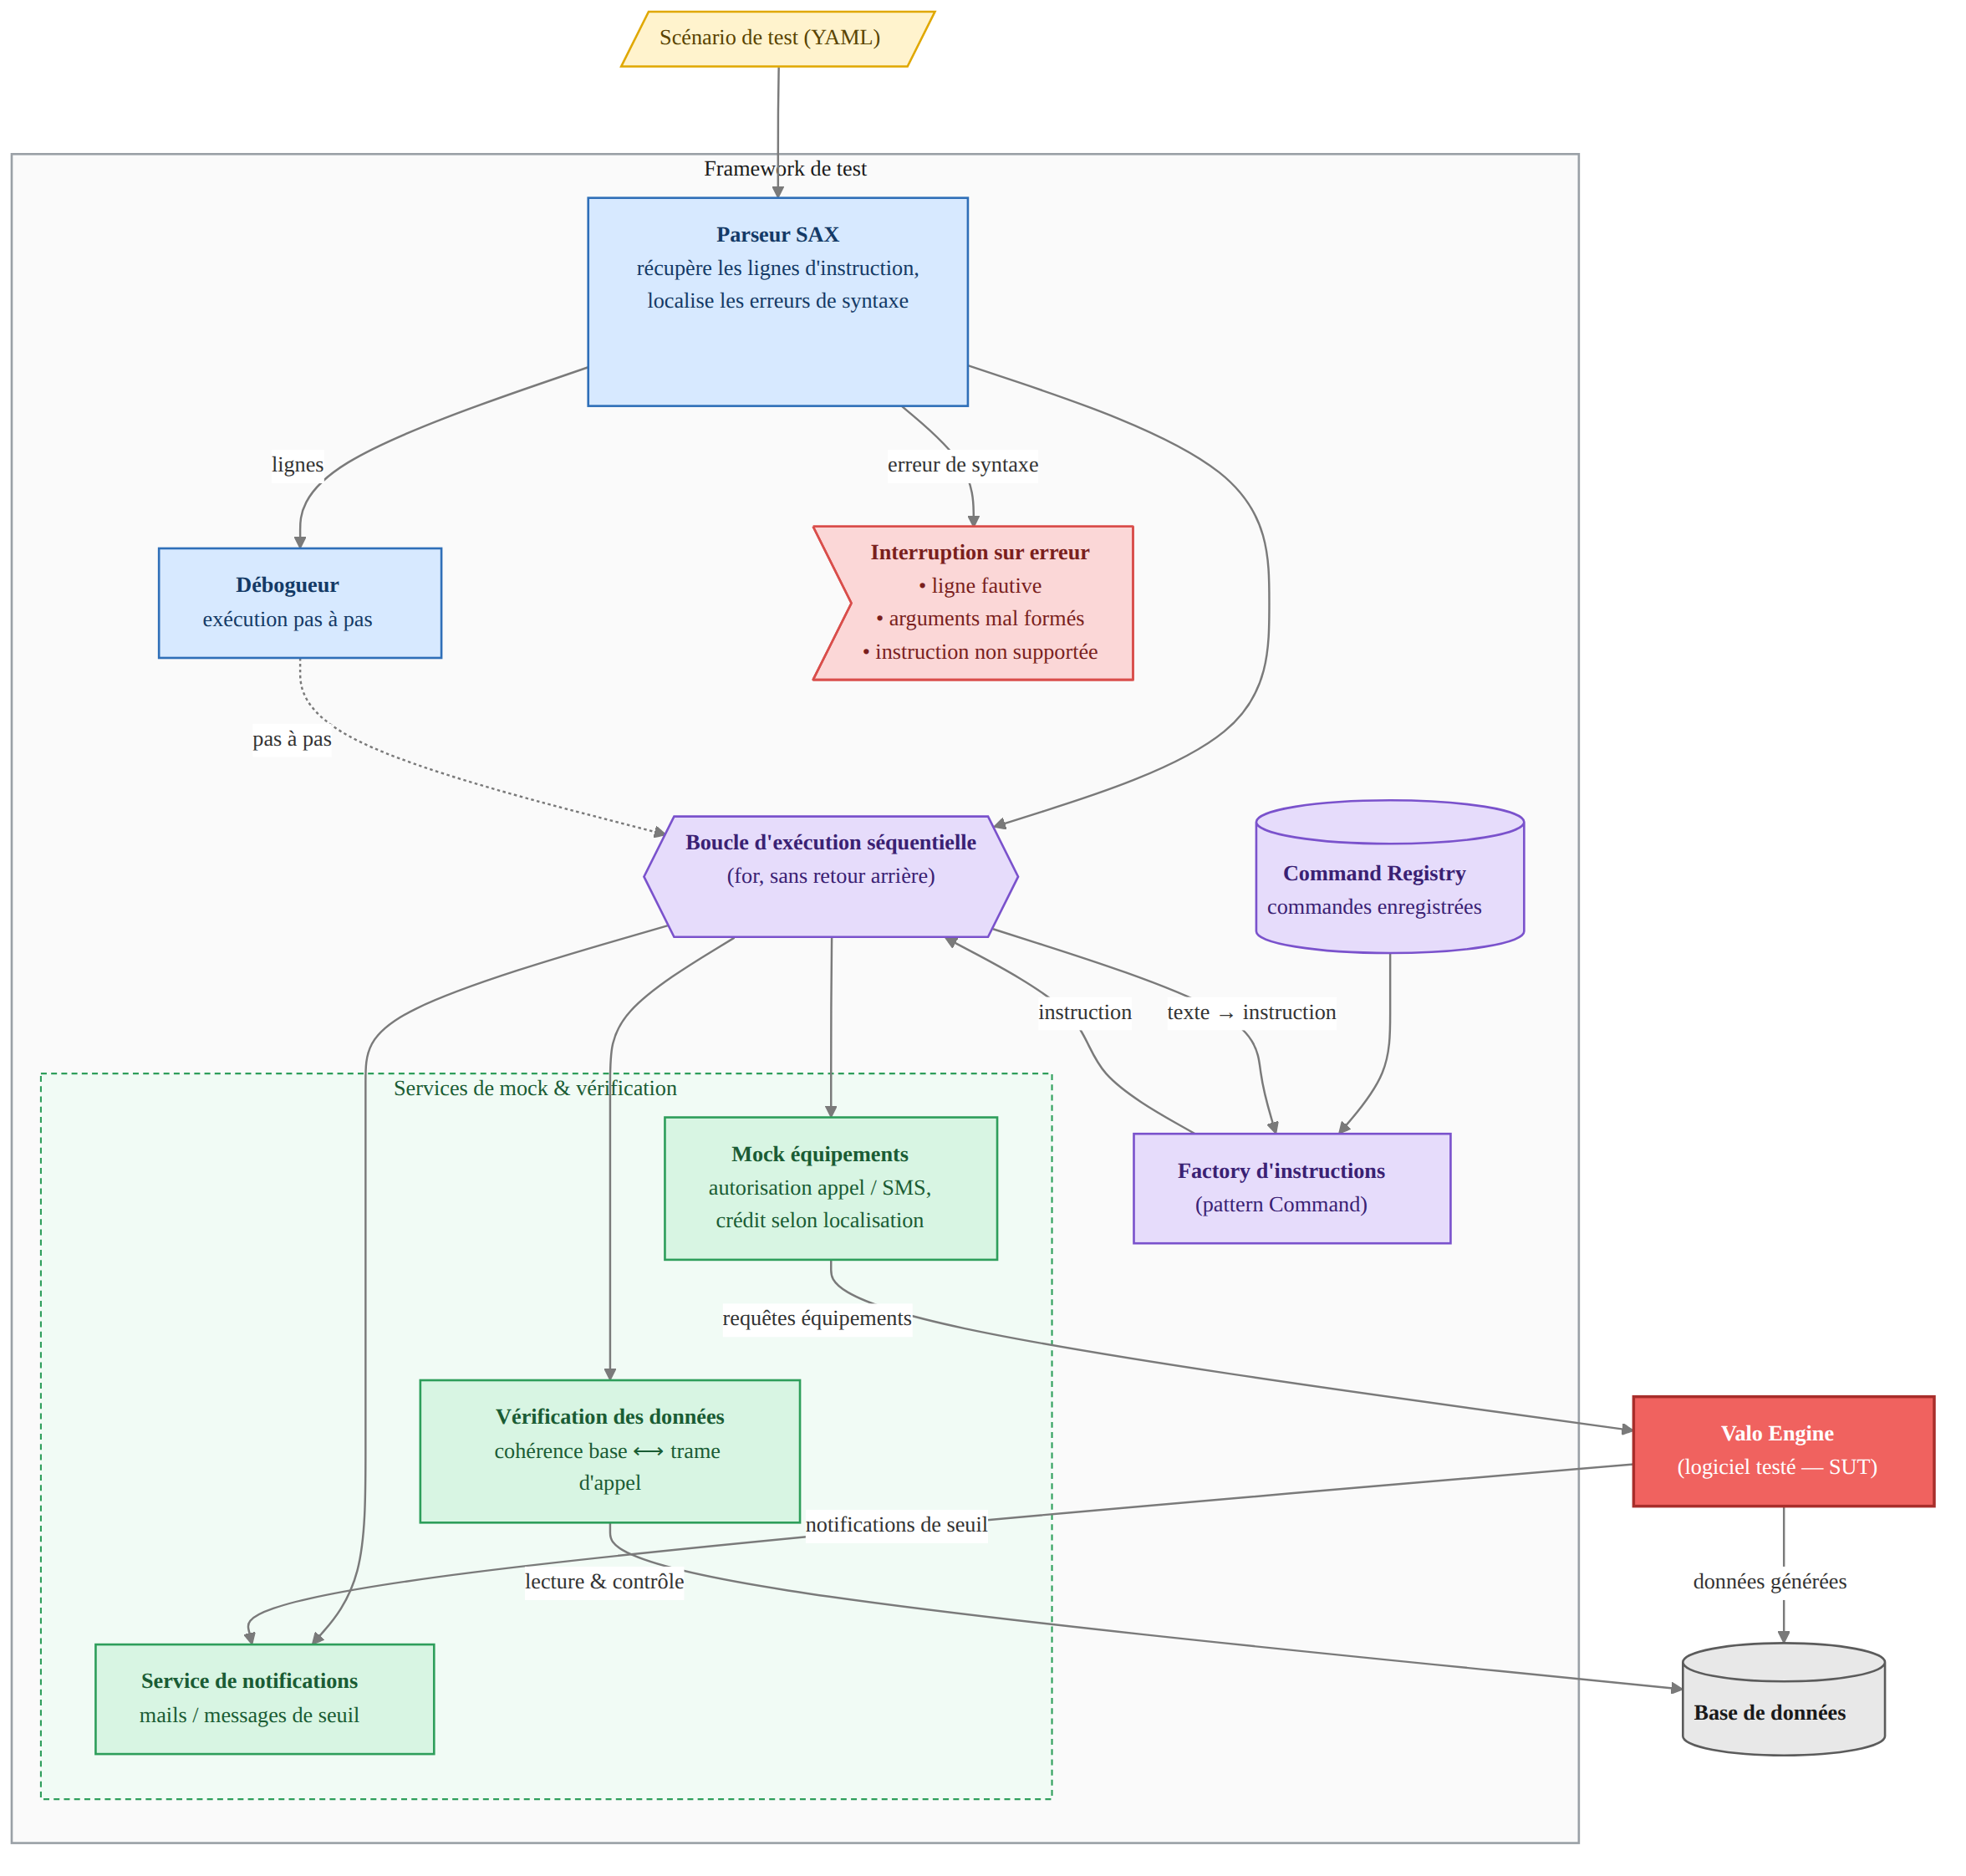
\includegraphics[width=\textwidth]{framework.png}
  \caption{Architecture du framework de test.}\label{fig:archi-t3}
\end{figure}

\section{Réalisation}
% TODO : illustrer par un EXTRAIT de code commenté (pas le code entier).
% Exemple de gabarit listing :
% \begin{lstlisting}[language=Python,caption={Définition d'un cas de test.},label={lst:t1}]
% def test_exemple():
%     ...
% \end{lstlisting}
\emph{[À rédiger.]}

\section{Difficultés rencontrées}
% TODO : ex. environnements non reproductibles, données de test, flakiness.
S'agissant de l'une des premières missions d'envergure qui m'étaient confiées,
la principale difficulté a tenu au \textbf{découpage du travail}. Plutôt que de
procéder par versions intermédiaires, livrables et vérifiables au fur et à
mesure, je me suis engagé d'emblée dans la conception complète d'une première
version couvrant l'ensemble des fonctionnalités du Lua. Ce choix a allongé le
délai avant d'obtenir un premier retour concret et m'a privé des points de
contrôle qu'un découpage plus fin aurait offerts.

Le second point, apparu avec le recul, concerne le choix de bâtir le framework
sur Pytest. Si cet outil fournit gratuitement un socle d'exécution et de
reporting éprouvé, il recèle aussi de nombreux mécanismes implicites — sa
« \emph{black magic} » — dont le comportement peut se révéler déroutant et
compliquer le développement d'une surcouche.

\section{Résultats et bénéfice business}
% TODO : couverture obtenue, régressions détectées, temps gagné,
% confiance dans les livraisons. Relier au chapitre \ref{chap:veille}.
\emph{[À rédiger.]}
